% =========================================================================
% PHẦN TRÊN: TIẾP TỤC VÍ DỤ 4 VÀ ĐỒ THỊ HÌNH 10
% =========================================================================
\noindent
\begin{minipage}[t]{0.28\textwidth}
    % Cột lề trái: Ghi chú đồ thị đường tròn béo, dóng ngang hàng với Hình 10
    \vspace*{142pt}
    {\small\noindent
    Hình 10 thể hiện đồ thị của đường cong $x^4 + y^4 = 16$ trong Ví dụ 4. Hãy để ý rằng đây là một phiên bản bị kéo giãn và làm phẳng của đường tròn $x^2 + y^2 = 4$. Vì lý do này, đôi khi nó được gọi là một \textit{đường tròn béo}. Đồ thị bắt đầu rất dốc ở bên trái nhưng nhanh chóng trở nên rất phẳng. Điều này có thể thấy rõ từ biểu thức
    \begin{equation*}
        y' = -\frac{x^3}{y^3} = -\left(\frac{x}{y}\right)^3
    \end{equation*}
    }
\end{minipage}%
\hfill
\begin{minipage}[t]{0.69\textwidth}
    % Cột chính: Tiếp tục giải đạo hàm cấp hai y''
    Để tìm $y''$, ta lấy đạo hàm biểu thức này của $y'$ bằng cách dùng Quy tắc thương và ghi nhớ rằng $y$ là một hàm số theo $x$:
    \begin{align*}
        y'' &= \frac{d}{dx}\left(-\frac{x^3}{y^3}\right) = -\frac{y^3(d/dx)(x^3) - x^3(d/dx)(y^3)}{(y^3)^2}\\[4pt]
        &= -\frac{y^3 \cdot 3x^2 - x^3(3y^2 y')}{y^6}
    \end{align*}
    Bây giờ nếu thay Phương trình 3 vào biểu thức này, ta được
    \begin{align*}
        y'' &= -\frac{3x^2 y^3 - 3x^3 y^2 \left(-\dfrac{x^3}{y^3}\right)}{y^6}\\[4pt]
        &= -\frac{3(x^2 y^4 + x^6)}{y^7} = -\frac{3x^2(y^4 + x^4)}{y^7}
    \end{align*}
    Nhưng các giá trị của $x$ và $y$ phải thỏa mãn phương trình ban đầu $x^4 + y^4 = 16$. Do đó kết quả được rút gọn thành
    \begin{equation*}
        y'' = -\frac{3x^2(16)}{y^7} = -48\frac{x^2}{y^7} \qquad {\color{stewartcyan}\rule{1.1ex}{1.1ex}}
    \end{equation*}

    \vspace{4pt}
    \begin{center}
        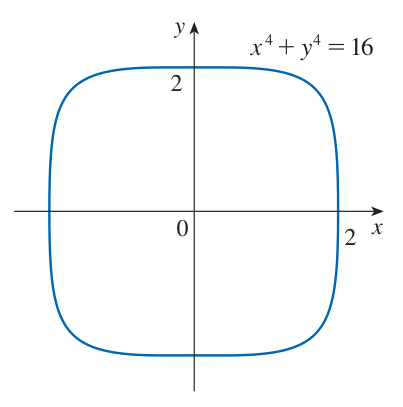
\includegraphics[width=0.48\linewidth]{images/p0249_fig1.png}\\[4pt]
        \textbf{\textsf{\small HÌNH 10}}
    \end{center}
\end{minipage}

\vspace{8pt}

% =========================================================================
% THANH TIÊU ĐỀ BÀI TẬP: 3.5 | BÀI TẬP
% =========================================================================
\noindent
\begin{tikzpicture}[x=\textwidth, y=1pt]
    \draw[stewartcyan, line width=0.6pt] (0, 4) -- (1, 4);
    \draw[stewartcyan, line width=0.6pt] (0, 1.5) -- (1, 1.5);
    \node[fill=white, inner sep=4pt, anchor=west] at (0.22, 2.75) {%
        \textbf{\textsf{\Large\color{stewartcyan}3.5}}\hspace{0.5em}%
        {\color{stewartcyan}\rule[-1.5pt]{1pt}{13pt}}\hspace{0.5em}%
        \textbf{\textsf{\Large BÀI TẬP}}%
    };
\end{tikzpicture}

\vspace{8pt}

% =========================================================================
% PHẦN DƯỚI: NỘI DUNG CÁC BÀI TẬP (CỘT LỀ: 1--8, CỘT CHÍNH: 9--24)
% =========================================================================
\noindent
\begin{minipage}[t]{0.28\textwidth}
    % Cột lề: Các bài tập 1 đến 8
    {\small
    \noindent\textbf{\textsf{\color{stewartcyan}1--4}}\\[2pt]
    (a) Tìm $y'$ bằng phương pháp đạo hàm ẩn.\\[2pt]
    (b) Giải phương trình tường minh theo $y$ và tính đạo hàm để nhận được $y'$ theo $x$.\\[2pt]
    (c) Kiểm tra xem các kết quả ở phần (a) và (b) có khớp nhau không bằng cách thay biểu thức của $y$ vào kết quả ở phần (a).\\[6pt]
    \noindent
    \begin{tabular*}{\linewidth}{@{}l@{\extracolsep{\fill}}l@{}}
        \textbf{1.} $5x^2 - y^3 = 7$ & \textbf{2.} $6x^4 + y^5 = 2x$ \\[6pt]
        \textbf{3.} $\sqrt{x} + \sqrt{y} = 1$ & \textbf{4.} $\dfrac{2}{x} - \dfrac{1}{y} = 4$
    \end{tabular*}

    \vspace{8pt}
    {\color{stewartcyan}\hrule height 0.6pt}
    \vspace{6pt}

    \noindent\textbf{\textsf{\color{stewartcyan}5--22}}\quad Tìm $dy/dx$ bằng phương pháp đạo hàm ẩn.\\[6pt]
    \noindent
    \begin{tabular*}{\linewidth}{@{}l@{\extracolsep{\fill}}l@{}}
        \textbf{5.} $x^2 - 4xy + y^2 = 4$ & \textbf{6.} $2x^2 + xy - y^2 = 2$ \\[6pt]
        \textbf{7.} $x^4 + x^2y^2 + y^3 = 5$ & \textbf{8.} $x^3 - xy^2 + y^3 = 1$
    \end{tabular*}
    }
\end{minipage}%
\hfill
\begin{minipage}[t]{0.69\textwidth}
    % Cột chính: Các bài tập 9 đến 24
    {\small
    \noindent
    \begin{tabular*}{\linewidth}{@{}p{0.48\linewidth}@{\extracolsep{\fill}}p{0.48\linewidth}@{}}
        \textbf{9.} $\dfrac{x^2}{x + y} = y^2 + 1$ & \textbf{10.} $xe^y = x - y$ \\[8pt]
        \textbf{11.} $\sin x + \cos y = 2x - 3y$ & \textbf{12.} $e^x \sin y = x + y$ \\[8pt]
        \textbf{13.} $\sin(x + y) = \cos x + \cos y$ & \textbf{14.} $\tan(x - y) = \dfrac{2x}{y + 1}$ \\[8pt]
        \textbf{15.} $y \cos x = x^2 + y^2$ & \textbf{16.} $\sin(xy) = \cos(x + y)$ \\[8pt]
        \textbf{17.} $2xe^y + ye^x = 3$ & \textbf{18.} $\sin x \cos y = x^2 - 5y$ \\[8pt]
        \textbf{19.} $\sqrt{x + y} = x^4 + y^4$ & \textbf{20.} $xy = \sqrt{x^2 + y^2}$ \\[8pt]
        \textbf{21.} $e^{x/y} = x - y$ & \textbf{22.} $\cos(x^2 + y^2) = xe^y$
    \end{tabular*}

    \vspace{10pt}
    \noindent\textbf{23.}\quad Nếu $f(x) + x^2 [f(x)]^3 = 10$ và $f(1) = 2$, hãy tìm $f'(1)$.\\[6pt]
    \noindent\textbf{24.}\quad Nếu $g(x) + x \sin g(x) = x^2$, hãy tìm $g'(0)$.
    }
\end{minipage}
